\chapter{Graph Algorithm}

\section{Definitions}
A \textbf{graph} is an important mathematical structure. A graph \(G = (V, E)\) consists of a set of vertices (or nodes) \(V\) and a set of edges \(E\). Each edge is a pair \((v, w)\), where \(v, w \in V\). Edges are sometimes referred to as \textit{arcs}.

If \(e = (v, w)\) is an edge with vertices \(v\) and \(w\), then \(v\) and \(w\) are said to \textit{lie on} \(e\), and \(e\) is said to be \textit{incident with} \(v\) and \(w\).

If the pairs are unordered, then \(G\) is called an \textbf{undirected graph}. If the pairs are ordered, then \(G\) is called a \textbf{directed graph}. The term \textit{directed graph} is often shortened to \textit{digraph}, and the unqualified term \textit{graph} usually refers to an undirected graph.

Vertex \(w\) is said to be \textit{adjacent to} vertex \(v\) if and only if \((v, w) \in E\). In an undirected graph, if \((v, w) \in E\), then \((w, v) \in E\) as well, so \(v\) is adjacent to \(w\) and \(w\) is adjacent to \(v\). Sometimes, an edge has a third component, known as either a \textit{weight} or a \textit{cost}.

A \textbf{path} in a graph is a sequence of vertices \(w_1, w_2, \ldots, w_n\) such that \((w_i, w_{i+1}) \in E\) for \(1 \leq i \leq n - 1\). The \textit{length} of such a path is the number of edges on the path, which is equal to \(n - 1\). 

We allow a path from a vertex to itself. If this path contains no edges, then the path length is 0. If the graph contains an edge \((v, v)\) from a vertex to itself, then the path \(v, v\) is sometimes referred to as a \textbf{loop}. 

A \textbf{simple path} is a path in which all vertices are distinct, except that the first and last vertices may be the same.

A cycle in a directed graph is a path of length at least 1 such that \(w_1 = w_n\). This cycle is called *simple* if the path is simple. For undirected graphs, we require that the edges be distinct. The logic behind this requirement is that the path \(u, v, u\) in an undirected graph should not be considered a cycle, because \((u, v)\) and \((v, u)\) represent the same edge. However, in a directed graph, these are different edges, so it makes sense to call this a cycle.

A directed graph is acyclic if it has no cycles. A directed acyclic graph is sometimes referred to by its abbreviation, DAG.

An undirected graph is connected if there is a path from every vertex to every other vertex. A directed graph with this property is called strongly connected. If a directed graph is not strongly connected, but the underlying graph (without direction to the arcs) is connected, then the graph is said to be weakly connected. A complete graph is a graph in which there is an edge between every pair of vertices.

\section{Implementation}
Consider each airport as a vertex, and two vertices are connected by an edge if there is a nonstop flight between the airports represented by the vertices. The edge could have a weight, representing the time, distance, or cost of the flight. Such a graph is directed, since it might take longer or cost more to fly in different directions.

We would like to make sure that the airport system is strongly connected, so that it is always possible to fly from any airport to any other airport. We might also like to quickly determine the best flight between any two airports. This could mean the path with the fewest number of edges or could be taken with respect to one or all of the weight measures.

To implement such a system, we can use a \textbf{two-dimensional array}. This is known as an \textbf{adjacency matrix representation}. For each \textbf{edge} \((u, v)\), we set \(a[u][v] = 1\), otherwise the entry in the array is 0. If the edge has a \textbf{weight} associated with it, then we can set \(a[u][v]\) equal to the weight and use either a very large or a very small weight as a \textbf{sentinel} to indicate \textbf{nonexistent edges}.

Then, if we were looking for the cheapest airplane route, we could represent nonexistent flights with a cost of \(\infty\). If we were somehow looking for the most expensive airplane route, we could use \(-\infty\) to represent nonexistent edges.

The space requirement is \(\Theta(\vert V \vert^2)\). This is unacceptable if the graph does not have many edges. An adjacency matrix is an appropriate representation if the graph is dense, \(\vert E \vert = \Theta(\vert V \vert^2)\).

However, if the graph is not dense but sparse, a better solution is an adjacency list representation. For each vertex, we keep a list of all adjacent vertices. The space requirement is then \(O(\vert E \vert + \vert V \vert)\). If the edges have weights, then this additional information is also stored in the cells. 

\section{Topological Sort}
A \textbf{topological sort} is a \textbf{linear ordering of vertices} in a \textbf{directed acyclic graph (DAG)} such that for every directed edge from vertex \(u\) to vertex \(v\), vertex \(u\) comes before vertex \(v\) in the ordering. A directed edge \((v, w)\) indicates that course \(v\) must be completed before course \(w\) may be attempted.

A topological ordering is then a linear sequence of the vertices such that for every directed edge from vertex \(u\) to vertex \(v\), \(u\) appears before \(v\) in the sequence. In other words, the ordering respects all the directed dependencies in the graph.

Notice that a topological ordering is not possible with a cyclic graph, since for two vertices \(v\) and \(w\) on the cycle, \(v\) precedes \(w\) and \(w\) precedes \(v\). The ordering is not necessarily unique; any valid ordering will suffice.

To find the topological ordering, we first define the \textbf{in-degree} of a vertex \(v\) as the number of incoming edges \((u, v)\). We compute the in-degrees of all vertices in the graph. Then, we find any vertex with an in-degree of zero, print this vertex, and remove it along with its outgoing edges from the graph. We then apply this same strategy to the rest of the graph. 

\begin{minipage}{0.5\textwidth}
  \begin{figure}[H]
    \centering
    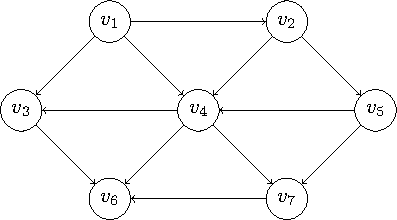
\includegraphics[width=0.8\textwidth]{Figure/topo_sort_demo.pdf}
    \caption{Topological Sort}
  \end{figure}
\end{minipage}
\begin{minipage}{0.5\textwidth}
  \begin{table}[H]
    \centering
    \begin{tabular}{c|c c c c c c c}
        \toprule
         & \multicolumn{7}{c}{In-degree before dequeue}  \\
      \midrule
        Vertex & 1 & 2 & 3 & 4 & 5 & 6 & 7  \\
      \midrule
        \(v_1\) & 0 & 0 & 0 & 0 & 0 & 0 & 0  \\
        \(v_2\) & 1 & 0 & 0 & 0 & 0 & 0 & 0  \\
        \(v_3\) & 2 & 1 & 1 & 1 & 0 & 0 & 0  \\
        \(v_4\) & 3 & 2 & 1 & 0 & 0 & 0 & 0  \\
        \(v_5\) & 1 & 1 & 0 & 0 & 0 & 0 & 0  \\
        \(v_6\) & 3 & 3 & 3 & 3 & 2 & 1 & 0  \\
        \(v_7\) & 2 & 2 & 2 & 1 & 0 & 0 & 0  \\
      \midrule
        \verb|enqueue| & \(v_1\) & \(v_2\) & \(v_5\) & \(v_4\) & \(v_3\) & \(v_7\) & \(v_6\)  \\
      \midrule
        \verb|dequeue| & \(v_1\) & \(v_2\) & \(v_5\) & \(v_4\) & \(v_3\) & \(v_7\) & \(v_6\)  \\
        \bottomrule
    \end{tabular}
    \caption{Topological Sorting}
  \end{table}
\end{minipage}

Since it is a simple sequential scan of the in-degree array, each call to it takes \(O(\vert V \vert)\) time. Since there are \(\vert V \vert\) such calls, the running time of the algorithm is \(O(\vert V \vert^2)\).

\section{Algorithms}
Here we introduce some algorithms that are related to graphs.

\subsection{Shortest Path Algorithm}
For the shortest path algorithm, the input is a weighted graph. Associated with each edge \((v_i, v_j)\) is a cost \(c_{i, j}\) to traverse the arc. The cost of a path \(v_1, v_2, \cdots, v_n\) is \(\sum_{i = 1}^{n - 1} c_{i, i + 1}\). This is referred to as the weighted path length. The unweighted path length is merely the number of edges on the path, namely \(n - 1\).

\begin{minipage}{0.5\textwidth}
  \begin{figure}[H]
    \centering
    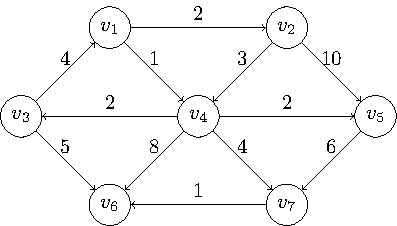
\includegraphics[width=0.7\textwidth]{Figure/shortest_path_algo.pdf}
    \caption{A weighted graph}
  \end{figure}
\end{minipage}\quad\quad
\begin{minipage}{0.5\textwidth}
  \begin{figure}[H]
    \centering
    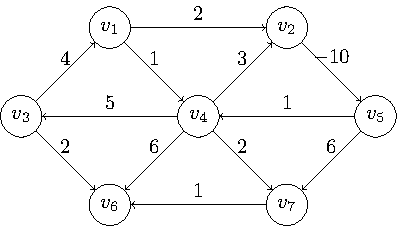
\includegraphics[width=0.7\textwidth]{Figure/ng_weight_path.pdf}
    \caption{A weighted graph}
  \end{figure}
\end{minipage}\quad\quad

For example, given as input a weighted graph \(G = (V, E)\) and a distinguished vertex \(s\), we are asked to find the shortest weighted path from \(s\) to every other vertex in \(G\).

In Figure 9.2, the shortest weighted path from \(v_1\) to \(v_6\) has a cost of 6 and goes from \(v_1\) to \(v_4\) to \(v_7\) to \(v_6\). The shortest unweighted path between these vertices has a length of 2. 

There could also be cases where the cost is negative. For example, in Figure 9.3, the path from \(v_5\) to \(v_4\) has cost 1, but a shorter path exists by following the loop \(v_5, v_4, v_2, v_5, v_4\), which has a cost of \(-5\). The shortest path between \(v_5\) and \(v_4\) is undefined. This loop is known as a negative-cost cycle. When one is present in the graph, the shortest paths are not defined.

Currently, there are no algorithms in which finding the path from \(s\) to one vertex is significantly faster (by more than a constant factor) than finding the paths from \(s\) to all vertices. The intermediate nodes in a shortest path must also lie on the shortest paths from \(s\).

If we assume that there are no negative edges, then for the weighted shortest path problem, the running time of the algorithm will be \(O(\vert E \vert \log \vert V \vert)\) when implemented with reasonable data structures.

If the graph has negative edges, we will have a poor time bound of \(O(\vert E \vert \cdot \vert V \vert)\). We will solve the weighted problem for the special case of acyclic graphs in linear time.

\subsection{Breadth-first Search}
We want to find the unweighted shortest path. Using vertex \(s\), we would like to find the shortest path from \(s\) to all other vertices. There are no weights on the edges, which is a special case of the weighted shortest-path problem, since we could assign all edges a weight of 1. 

We can use \textbf{breadth-first search (BFS)} to search for the shortest path. It operates by processing vertices in layers. The vertices closest to the start are evaluated first, and the most distant vertices are evaluated last. This is much the same as a level-order traversal for trees.



For each vertex, we will keep track of three pieces of information. First, we will keep its distance from \(s\) in the entry \(d_v\). Initially, all vertices are unreachable except for \(s\), whose path length is 0. The entry in \(p_v\) is the bookkeeping variable, which will allow us to print the actual paths. The entry \texttt{known} is set to 1 after a vertex is processed. Initially, all entries are unknown, including the start vertex. Once it is known, we have a guarantee that no cheaper path will ever be found, and so processing for that vertex is essentially complete.

In Figure 9.4, suppose we choose \(s\) to be \(v_3\). The shortest path from \(s\) to \(v_3\) is then a path of length 0. Now we can start looking for all vertices that are a distance 1 away from \(s\). These can be found by looking at the vertices that are adjacent to \(s\). Then we have

\begin{minipage}{0.33\textwidth}
  \begin{figure}[H]
    \centering
    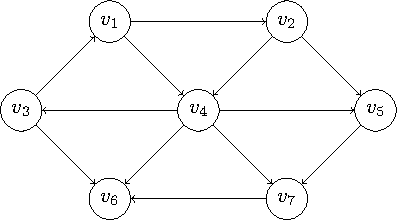
\includegraphics[width=\textwidth]{Figure/unweighted_path.pdf}
    \caption{Unweighted graph}
  \end{figure}
\end{minipage}
\begin{minipage}{0.33\textwidth}
\begin{table}[H]
  \centering
  \begin{tabular}{c|c|c|c}
      \toprule
      \verb|v| & Known & \(d_v\) & \(p_v\)  \\
    \midrule
      \(v_1\) & 0 & \(\infty\) & 0  \\
      \(v_2\) & 0 & \(\infty\) & 0  \\
      \(v_3\) & 0 & \(0\) & 0  \\
      \(v_4\) & 0 & \(\infty\) & 0  \\
      \(v_5\) & 0 & \(\infty\) & 0  \\
      \(v_6\) & 0 & \(\infty\) & 0  \\
      \(v_7\) & 0 & \(\infty\) & 0  \\
    \midrule
      \verb|Q| & \multicolumn{3}{c}{\(v_3\)} \\
    \bottomrule
  \end{tabular}
  \caption*{Initial State}
\end{table}
\end{minipage}
\begin{minipage}{0.33\textwidth}
  \begin{table}[H]
    \centering
    \begin{tabular}{c|c|c|c}
        \toprule
        \verb|v| & Known & \(d_v\) & \(p_v\)  \\
      \midrule
        \(v_1\) & 0 & 1 & \(v_3\)  \\
        \(v_2\) & 0 & \(\infty\) & 0  \\
        \(v_3\) & 1 & 0 & 0  \\
        \(v_4\) & 0 & \(\infty\) & 0  \\
        \(v_5\) & 0 & \(\infty\) & 0  \\
        \(v_6\) & 0 & 1 & \(v_3\)  \\
        \(v_7\) & 0 & \(\infty\) & 0  \\
      \midrule
        \verb|Q| & \multicolumn{3}{c}{\(v_1, v_6\)} \\
      \bottomrule
    \end{tabular}
    \caption*{\(v_3\) dequeued}
  \end{table}
\end{minipage}

\begin{minipage}{0.33\textwidth}
  \begin{table}[H]
    \centering
    \begin{tabular}{c|c|c|c}
        \toprule
        \verb|v| & Known & \(d_v\) & \(p_v\)  \\
      \midrule
        \(v_1\) & 1 & 1 & \(v_3\)  \\
        \(v_2\) & 0 & 2 & \(v_1\)  \\
        \(v_3\) & 1 & 0 & 0  \\
        \(v_4\) & 0 & 2 & \(v_1\)  \\
        \(v_5\) & 0 & \(\infty\) & 0  \\
        \(v_6\) & 0 & 1 & \(v_3\)  \\
        \(v_7\) & 0 & \(\infty\) & 0  \\
      \midrule
        \verb|Q| & \multicolumn{3}{c}{\(v_6, v_2, v_4\)} \\
      \bottomrule
    \end{tabular}
    \caption*{\(v_1\) dequeued}
  \end{table}
\end{minipage}
\begin{minipage}{0.33\textwidth}
  \begin{table}[H]
    \centering
    \begin{tabular}{c|c|c|c}
        \toprule
        \verb|v| & Known & \(d_v\) & \(p_v\)  \\
      \midrule
        \(v_1\) & 1 & 1 & \(v_3\)  \\
        \(v_2\) & 0 & 2 & \(v_1\)  \\
        \(v_3\) & 1 & 0 & 0  \\
        \(v_4\) & 0 & 2 & \(v_1\)  \\
        \(v_5\) & 0 & \(\infty\) & 0  \\
        \(v_6\) & 1 & 1 & \(v_3\)  \\
        \(v_7\) & 0 & \(\infty\) & 0  \\
      \midrule
        \verb|Q| & \multicolumn{3}{c}{\(v_2, v_4\)} \\
      \bottomrule
    \end{tabular}
    \caption*{\(v_6\) dequeued}
  \end{table}
\end{minipage}
\begin{minipage}{0.33\textwidth}
  \begin{table}[H]
    \centering
    \begin{tabular}{c|c|c|c}
        \toprule
        \verb|v| & Known & \(d_v\) & \(p_v\)  \\
      \midrule
        \(v_1\) & 1 & 1 & \(v_3\)  \\
        \(v_2\) & 1 & 2 & \(v_1\)  \\
        \(v_3\) & 1 & 0 & 0  \\
        \(v_4\) & 0 & 2 & \(v_1\)  \\
        \(v_5\) & 0 & 3 & \(v_2\)   \\
        \(v_6\) & 1 & 1 & \(v_3\)  \\
        \(v_7\) & 0 & \(\infty\) & 0  \\
      \midrule
        \verb|Q| & \multicolumn{3}{c}{\(v_4, v_5\)} \\
      \bottomrule
    \end{tabular}
    \caption*{\(v_2\) dequeued}
  \end{table}
\end{minipage}

\begin{minipage}{0.33\textwidth}
  \begin{table}[H]
    \centering
    \begin{tabular}{c|c|c|c}
        \toprule
        \verb|v| & Known & \(d_v\) & \(p_v\)  \\
      \midrule
        \(v_1\) & 1 & 1 & \(v_3\)  \\
        \(v_2\) & 1 & 2 & \(v_1\)  \\
        \(v_3\) & 1 & 0 & 0  \\
        \(v_4\) & 1 & 2 & \(v_1\)  \\
        \(v_5\) & 0 & 3 & \(v_2\)   \\
        \(v_6\) & 1 & 1 & \(v_3\)  \\
        \(v_7\) & 0 & 3 & \(v_4\)  \\
      \midrule
        \verb|Q| & \multicolumn{3}{c}{\(v_5, v_7\)} \\
      \bottomrule
    \end{tabular}
    \caption*{\(v_4\) dequeued}
  \end{table}
\end{minipage}
\begin{minipage}{0.33\textwidth}
  \begin{table}[H]
    \centering
    \begin{tabular}{c|c|c|c}
        \toprule
        \verb|v| & Known & \(d_v\) & \(p_v\)  \\
      \midrule
        \(v_1\) & 1 & 1 & \(v_3\)  \\
        \(v_2\) & 1 & 2 & \(v_1\)  \\
        \(v_3\) & 1 & 0 & 0  \\
        \(v_4\) & 1 & 2 & \(v_1\)  \\
        \(v_5\) & 1 & 3 & \(v_2\)   \\
        \(v_6\) & 1 & 1 & \(v_3\)  \\
        \(v_7\) & 0 & 3 & \(v_4\)  \\
      \midrule
        \verb|Q| & \multicolumn{3}{c}{\(v_7\)} \\
      \bottomrule
    \end{tabular}
    \caption*{\(v_5\) dequeued}
  \end{table}
\end{minipage}
\begin{minipage}{0.33\textwidth}
  \begin{table}[H]
    \centering
    \begin{tabular}{c|c|c|c}
        \toprule
        \verb|v| & Known & \(d_v\) & \(p_v\)  \\
      \midrule
        \(v_1\) & 1 & 1 & \(v_3\)  \\
        \(v_2\) & 1 & 2 & \(v_1\)  \\
        \(v_3\) & 1 & 0 & 0  \\
        \(v_4\) & 1 & 2 & \(v_1\)  \\
        \(v_5\) & 1 & 3 & \(v_2\)   \\
        \(v_6\) & 1 & 1 & \(v_3\)  \\
        \(v_7\) & 1 & 3 & \(v_4\)  \\
      \midrule
        \verb|Q| & \multicolumn{3}{c}{} \\
      \bottomrule
    \end{tabular}
    \caption*{\(v_7\) dequeued}
  \end{table}
\end{minipage}

The running time for this algorithm is \(O(\vert V \vert^2)\), because of the doubly nested \texttt{for} loops.

\subsection{Dijkstra's Algorithm}